\chapter{Generic scalar PDE on 3D angle domain}

\modinfo{Directory}{ModelPDE3D}
\modinfo{Solvers}{\Idx{ModelPDE}} 
\modinfo{Tools}{\Idx{ElmerGUI}} 
\modinfo{Dimensions}{3D, Steady-state}
\modinfo{Author}{Peter R{\aa}back}


\subsection*{Problem description}

This tutorial demonstrates the use of the generic advection-diffusion-reaction 
equation through ElmerGUI. The solver may be found in module ModelPDE. 
The purposes of the model pde and also this tutorial is to help 
those who want to understand Elmer from a mathematical perspective to be
able to carry out some of their own code development. 

The problem is a simple 3d structure \texttt{winkel.grd} that can be characterized by a 
$2\times 2\times 2$ topological grid where entries $(1,1,1)$, $(1,2,1)$, $(2,1,1)$ and
$(2,1,2)$ are meshed. This is the simplest Cartesian structure with full 3D 
solution. 

We can rather freely play with the parameters of the Model PDE. The equation is 
generic and the parameters are assumed to be unit free. 
For detailed description of the problem see the description in Elmer Programmers Tutorial.

As a first suggestion, we will show how to make a simple case where the two extreme edges 
are set to zero using Dirichlet boundary conditions, and constant unity source term is 
applied to the body. This is the simple Poisson equation with constant coefficient. 

\subsection*{Menu structures for Model PDE}

The menu structures for the case are defined in \texttt{model-pde.xml}. If after starting
you cannot find the menu structures add the file to the \texttt{edf} directory of your installation,
or append the menu structures within ElmerGUI. 

\noindent 
The following material parameters may be defined
\sifbegin
\sifitem{Diffusion Coefficient}{Real}
Diffusion coefficient, $\mu$.
\sifitem{Reaction Coefficient}{Real}
Reaction coefficient, $\lambda$.
\sifitem{Time Derivative Coefficient}{Real}
Multiplier of the time derivative, $\rho$.
\sifitem{Convection Coefficient}{Real}
Multiplier of convection coefficient, $\kappa$.
\sifitem{Convection Velocity 1}{Real}
Convection velocity in direction $x$, $a_x$.
\sifitem{Convection Velocity 2}{Real}
Convection velocity in direction $y$, $a_y$.
\sifitem{Convection Velocity 3}{Real}
Convection velocity in direction $z$, $a_z$.
\sifend

\noindent
The following parameter defines the heat source $f$ on the right-hand-side
\sifbegin
\sifitemnt{Field Source}{Real}
\sifend

\noindent
The menu structures defines the following parameters for boundary conditions:
\sifbegin
\sifitem{Field}{Real}
Dirichlet BC for the scalar field under study, $u$.
\sifitem{Field Flux}{Real}
Neumann boundary condition for the field, $q$.
\sifitemnt{Robin Coeffficient}{Real}
\sifitem{External Field}{Real}
Coefficient $\alpha$ and external field value $g$ for Robin boundary condition.
\sifend

\noindent
In transient cases the user may also give an initial condition for $u$, 
\sifbegin
\sifitemnt{Field}{Real}
\sifend


\subsection*{Solution procedure}

Start \texttt{ElmerGUI} from command line or by clicking the icon in your desktop. Here we describe 
the essential steps in the ElmerGUI by writing out the clicking procedure. Indentation generally means 
that the selections are done within the window chosen at the higher level. 

The mesh is given in ElmerGrid format in file \texttt{winkel.grd} in the samples directory of ElmerGUI, 
load this file.
\ttbegin
File 
  Open -> winkel.grd
\ttend
You should obtain your mesh and may check in the \texttt{Model summary} 
window that it consists of 35\,721 nodes and 32\,000 trilinear elements.
If the mesh was successfully imported your window should look something in figure~\ref{fg:modelpde1}.
The figure also shows the two extreme boundary patches that we intend to use Dirichlet conditions
for. 
\begin{figure}
\begin{center}
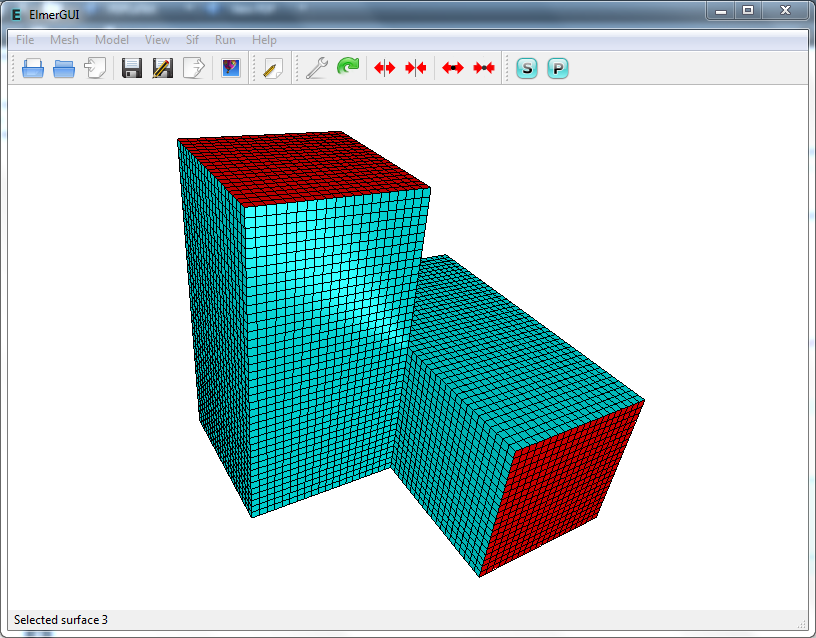
\includegraphics[width=100mm]{ModelPDE_Mesh.PNG}
\caption{The finite element mesh in ElmerGUI}\label{fg:modelpde1}
\end{center}
\end{figure}

After we have the mesh we start to go through the Model menu from the top to bottom. 
In the \texttt{Setup} we choose things related to the whole simulation such as file names, 
time stepping, constants etc.  The simulation is carried out in 2-dimensional Cartesian
coordinates and in steady-state. Only one steady-state iteration is needed as the case is linear. 
\ttbegin
Model
  Setup 
    Simulation Type = Steady state
    Steady state max. iter = 1
\ttend
Choose \texttt{Apply} to close the window.

In the equation section we choose the relevant equations and parameters related to their solution. 
In this case we'll have one set only one equation -- the Model PDE.


When defining Equations and Materials it is possible to assign to the bodies immediately, or to use mouse
selection to assign them later. In this case we have just one body and one boundary and therefore its easier to assign 
the Equation and Material to it directly.

For the linear system solvers we are happy to use the defaults. One may however, try out different
preconditioners (ILU1,\ldots) or direct Umfpack solver, for example.
\ttbegin
Model
  Equation
    Add 
      Name = Model PDE
      Apply to bodies = 1
      Model PDE
        Active = on
  Add   
  OK
\ttend        

The Material section includes all the material parameters.
If material parameter is not defined. It is assumed to be zero. 
Here we just set the diffusivity to one.
\ttbegin
Model
  Material
      Name = Ideal
      Apply to bodies = 1 
      Model PDE
        Diffusion Coefficient = 1.0
    Add
    OK
\ttend

A Body Force represents the right-hand-side of a equation,  
\ttbegin
Model
  Body Force
      Name = Source
      Apply to bodies = 1
      Model PDE
        Field Source = 1.0
    Add
    OK
\ttend    

No initial conditions are required in steady state case.

Finally, for the BCs first define them and then use the mouse to apply them to the correct
boundary patches.  Refer to figure~\ref{fg:modelpde1} and select the two surfaces as shown.
\ttbegin
Model
  BoundaryCondition
      Name = Zero
      Model PDE
        Field = 0.0
    Add
    OK
\ttend   


For the execution ElmerSolver needs the mesh files and the command file. We have now basically defined
all the information for ElmerGUI to write the command file. After writing it we may also visually 
inspect the command file.
\ttbegin
Sif 
  Generate
  Edit -> look how your command file came out  
\ttend

Before we can execute the solver we should save the files in a directory. In saving the project all the
necessary files for restarting the case will be saved to the 
destination directory.
\ttbegin
File 
  Save Project
\ttend

After we have successfully saved the files we may start the solver
\ttbegin
Run
  Start solver
\ttend
A convergence view automatically pops up showing relative changes of each iteration.
As the case is linear only one iteration was required for the solution and the second one
just is needed to check the convergence. 

The norm of the results at convergence should be 1.4243820.

Note: if you face problems in the solution phase and need to edit the setting, always remember to save
the project before execution.

To view the results we may visualize them with Paraview.

\begin{figure}
\begin{center}
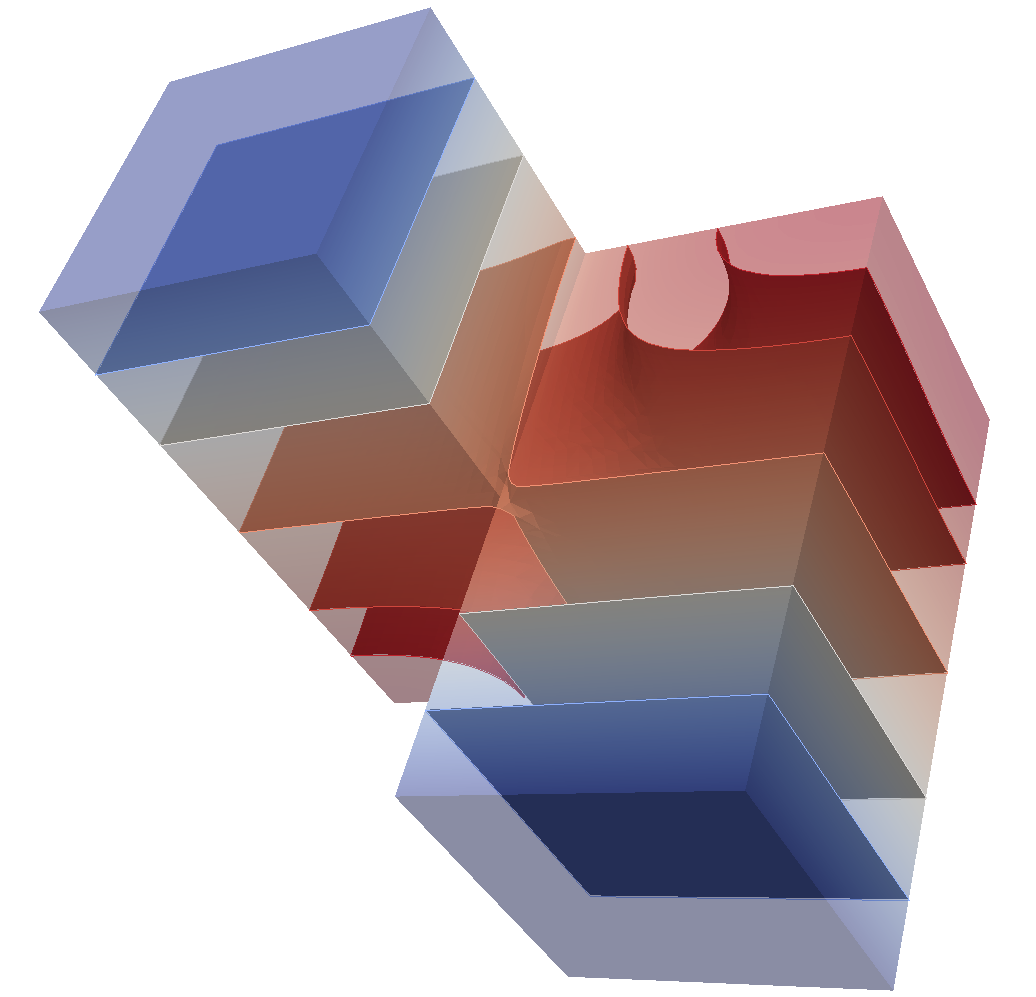
\includegraphics[width=100mm]{ModelPDE_Sol}
\caption{The field values of the structure as visualized with Paraview. Isosurfaces are 
defined for field values 0.5, 1.0, 1.5, 1.8 and 1.9, respectively.}\label{fg:post1}
\end{center}
\end{figure}


\subsection*{Further possibilities}

Here are some things you could try out, or are at least possible. The menus of the GUI are just 
elementary so more advanced features may need that the keywords are added by hand to the 
command file. No coding is needed to implement these features though. 
\begin{itemize}
\item You can also solve the problem with an unstructured tetrahedral mesh 
using Gmsh format file \texttt{winkel.msh}. 
\item Play with the reaction, diffusion, convection coefficient, and also the advection velocity.
As far as they remain constant the equation should be solvable with one sweep.
\item You could try to use Neumann or Robin BCs as well. Remember though that
a steady state equation needs definitions that uniquely define the solution.
\item Make the problem time-dependent. Note that then you most likely need to define the 
coefficient for the time derivative. 
\item When the advection increases in size the solution may eventually become oscillatory.
To eliminate that some bubbles or p-elements may be needed. You may play around with 
element settings, for example use \texttt{Element = p:2} or \texttt{Element = n:1 b:1} etc. 
\item You could try to increase the number of elements either by using \texttt{-relh} 
parameter in ElmerGUI, or setting \texttt{Mesh Levels = 2} in Simulation section.
\item You could try to use \texttt{MATC} to make the coefficients parameter dependent.
Dependence on the solution itself introduces non-linearities that might not be well handled 
by the fixed point iteration scheme. For more demanding non-linearities Newton linearisation or
other techniques may be needed. 
\item Also some periodicity could be introduced to this problem by letting the 
two extreme surface patches have a dependence between them.
\item You could introduce sort of contact conditions for the surface or bulk values 
of the problem by defining minimum or maximum values for the field. 
\end{itemize}


\hfill
\mbox{}






